%---------------------------------------------------------------------------
%   PACKAGES AND OTHER DOCUMENT CONFIGURATIONS
%---------------------------------------------------------------------------
\documentclass[final]{beamer}
\usepackage{gensymb}
\usepackage{textcomp}
\usepackage[scale=1.24, orientation=portrait]{beamerposter} % Use the beamerposter package for laying out the poster
\usetheme{confposter} % Use the confposter theme supplied with this template
\setbeamercolor{block title}{fg=purple,bg=white} % Colors of the block titles
\setbeamercolor{block body}{fg=black,bg=white} % Colors of the body of blocks
\setbeamercolor{block alerted title}{fg=white,bg=white} % Colors of the highlighted block titles
\setbeamercolor{block alerted body}{fg=black,bg=white!10} % Colors of the body of highlighted blocks
% Many more colors are available for use in beamerthemeconfposter.sty
%---------------------------------------------------------------------------
% Define the column widths and overall poster size
% To set effective sepwid, onecolwid and twocolwid values, first choose how many columns you want and how much separation you want between columns
% In this template, the separation width chosen is 0.024 of the paper width and a 4-column layout
% onecolwid should therefore be (1-(# of columns+1)*sepwid)/# of columns e.g. (1-(4+1)*0.024)/4 = 0.22
% Set twocolwid to be (2*onecolwid)+sepwid = 0.464
% Set threecolwid to be (3*onecolwid)+2*sepwid = 0.708
\newlength{\sepwid}
\newlength{\onecolwid}
\newlength{\twocolwid}
\newlength{\threecolwid}
\setlength{\paperwidth}{36in} % A0 width: 46.8in
\setlength{\paperheight}{48in} % A0 height: 33.1in
\setlength{\sepwid}{0.024\paperwidth} % Separation width (white space) between columns
\setlength{\onecolwid}{0.22\paperwidth} % Width of one column
\setlength{\twocolwid}{0.464\paperwidth} % Width of two columns
\setlength{\threecolwid}{0.708\paperwidth} % Width of three columns
\setlength{\topmargin}{-0.75in} % Reduce the top margin size
%---------------------------------------------------------------------------
\usepackage{graphicx}  % Required for including images
\usepackage{booktabs} % Top and bottom rules for tables
\graphicspath{{../plots/}}
%---------------------------------------------------------------------------
%   TITLE SECTION 
%---------------------------------------------------------------------------
\title{Measuring $^{nat}$La(p,x) Cross Sections from 35-60 MeV by Stacked Foil Activation} % Poster title
\author{$^1$Jonathan Morrell$^*$, $^1$Andrew Voyles, $^{1,2}$Lee Bernstein, $^2$Shamsuzzoha Basunia} % Author(s)
\institute{1: Nuclear Engineering, University of California, Berkeley\\
2: Lawrence Berkeley National Laboratory
} % Institution(s)
%----------------------------------------------------------------------------
\begin{document}
\addtobeamertemplate{headline}{} 

\begin{frame}[t] % The whole poster is enclosed in one beamer frame
\begin{columns}[t] % The whole poster consists of three major columns, the second of which is split into two columns twice - the [t] option aligns each column's content to the top
\begin{column}{\sepwid}\end{column} % Empty spacer column
\begin{column}{\onecolwid} % The first column
%----------------------------------------------------------------------------
%   LEFT
%---------------------------------------------------------------------------
\begin{block}{Introduction}
\small{\hspace*{50pt}Proton induced nuclear reactions in the tens of MeV range can be used for the production of radioactive isotopes with minimal contaminants, which makes them a compelling production mechanism for medical diagnostic and therapeudic isotopes \cite{TARKANYI2016262, nuclear_data_needs}.

\hspace*{50pt}In this experiment, we measure the $^{nat}$La(p,x) reaction cross sections with a particular interest in the (p,6n) reaction on $^{139}$La (99.9119\% n.a.) \cite{ensdf} for the production of $^{134}$Ce. 
}

\end{block}

\begin{block}{Methodology}


\small{\hspace*{50pt}Measurement of these reaction cross sections was performed using the stacked foil activation method:

\begin{itemize}
\item Calibrate the HPGe $\gamma$-ray detector
\item Measure the mass and dimensions of the target foils
\item Assemble the stack and secure in the beamline

\begin{figure}
\fbox{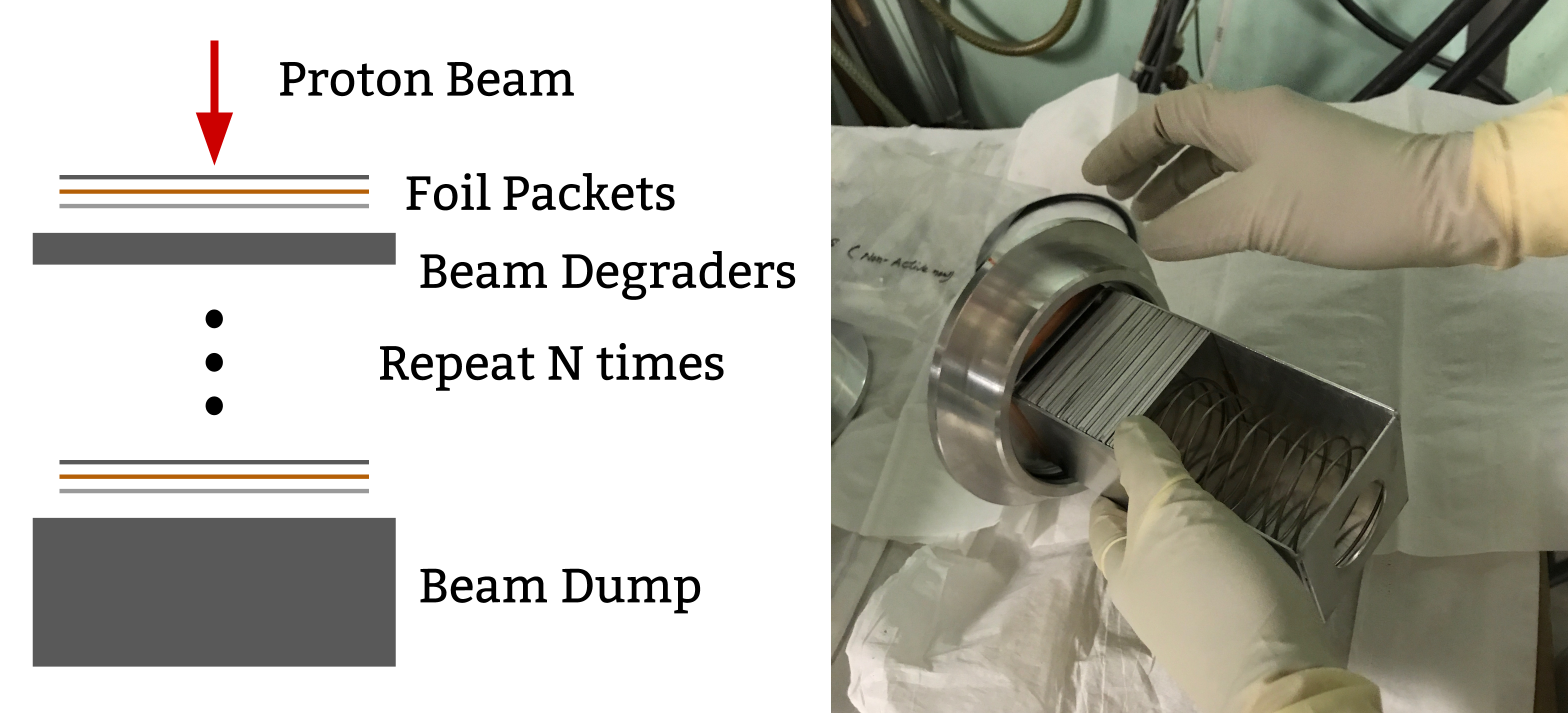
\includegraphics[width=0.8\linewidth]{photos/schematic_stack.png}}
\caption{\hspace*{15pt}Schematic of the foil stack (left) and photograph of stack prior to irradiation (right).}
\end{figure}

\item Irradiate for fixed duration and proton current
\item Count irradiated foils with HPGe detector
\item Fit peaks in the monitor and target foil spectra (Fig. 2)

\begin{figure}
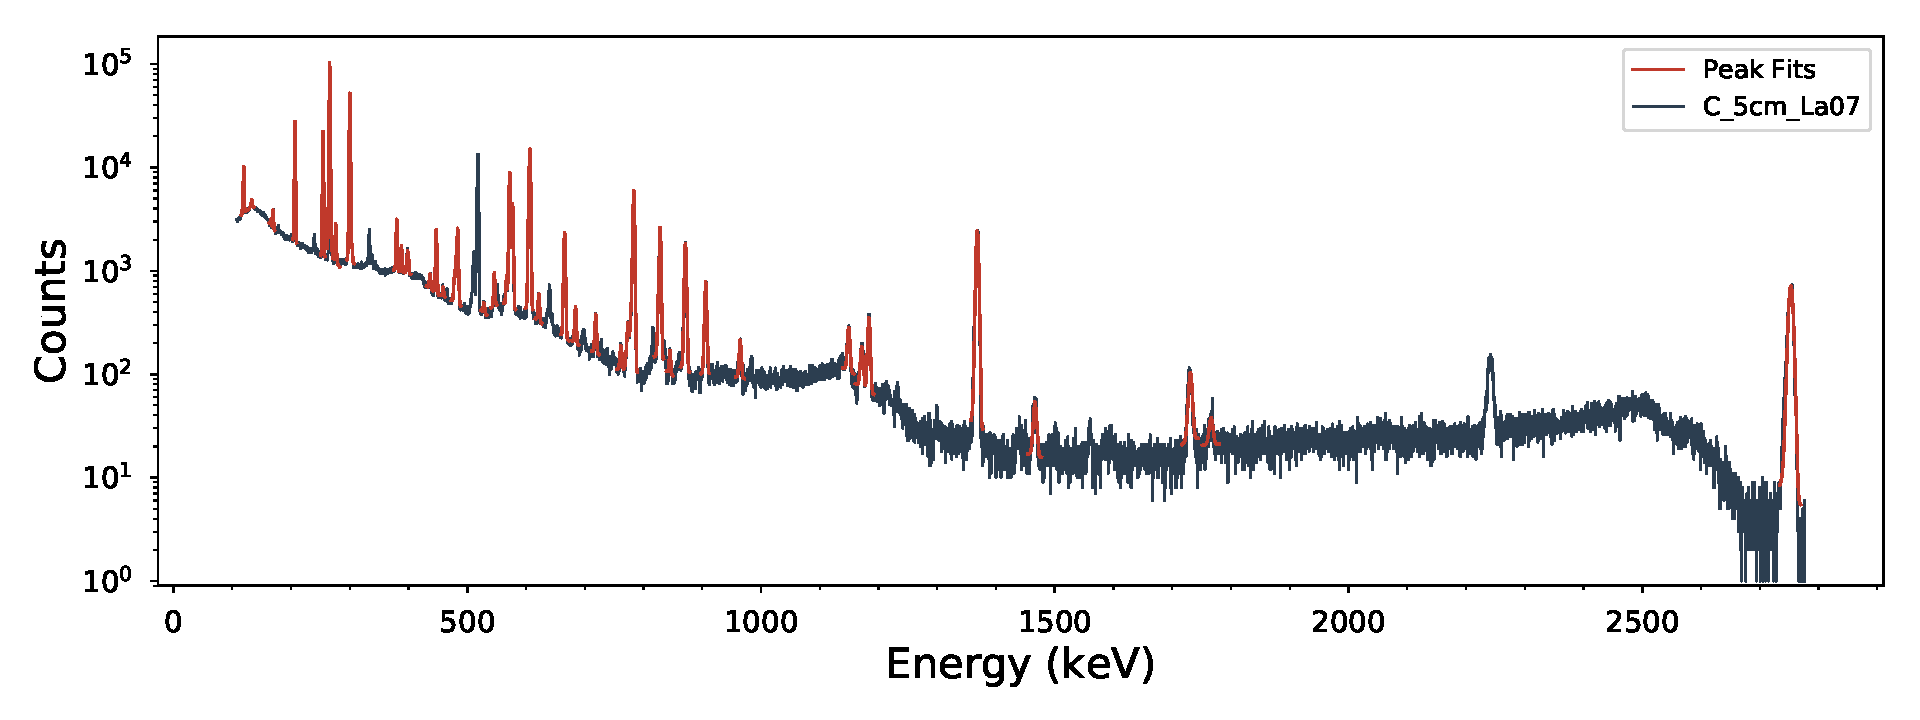
\includegraphics[width=0.9\linewidth]{peak_fits/C_5cm_La07_fits.pdf}
\caption{\hspace*{15pt}Example of $\gamma$-ray spectrum from the 7$^{th}$ lanthanum foil, with peak fits indicated in red.}
\end{figure}


\item Determine end-of-beam activities ($A_0$) in each foil
\item Determine beam current and energies
\item Calculate cross-sections
\item Compare results to EXFOR, TALYS, EMPIRE, and ALICE
\end{itemize}

}



\begin{block}{Data Analysis}
\small{\hspace*{50pt}The cross section can be determined by the indiced activity of a reaction product using the following equation:

\begin{equation}
\sigma =  A_0[I_p \rho \Delta r (1-e^{-\lambda t_i})]^{-1}
\label{eq:xs_calc}
\end{equation}

where $A_0$ is the activity of a given reaction product (at the end of irradiation), $I_p$ is the proton beam current, $\rho \Delta r$ is the areal number density. The factor $(1-e^{-\lambda t_i})$ is the ratio of induced activity to the saturation activity, where $\lambda$ is the decay constant for a given reaction product and $t_i$ is the total irradiation time. 

}
\end{block}


\end{block}

%----------------------------------------------------------------------------
\end{column} % End of the first column
\begin{column}{\sepwid}\end{column} % Empty spacer column
\begin{column}{\threecolwid} % Begin a column which is two columns wide (column 2)
%----------------------------------------------------------------------------
%        MIDDLE
%----------------------------------------------------------------------------

\begin{figure}
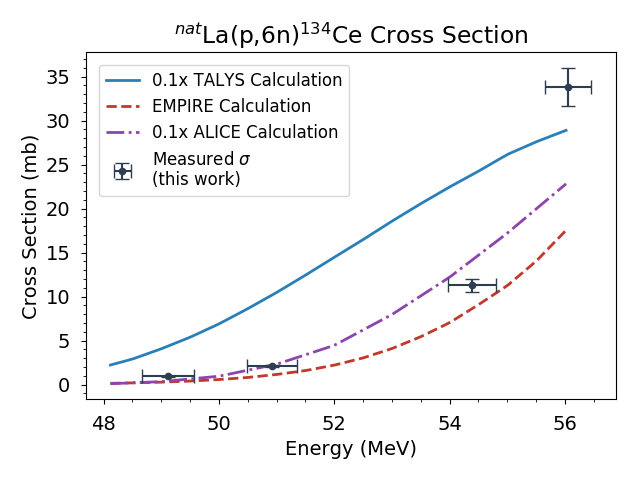
\includegraphics[width=0.32\linewidth]{cross_sections/134CE.png}
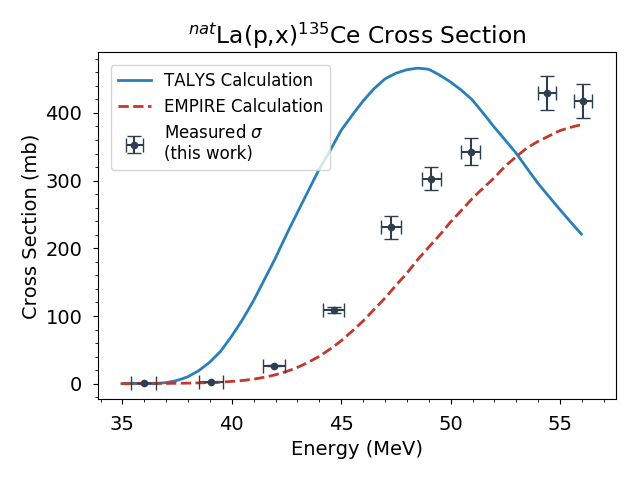
\includegraphics[width=0.32\linewidth]{cross_sections/135CE.png}
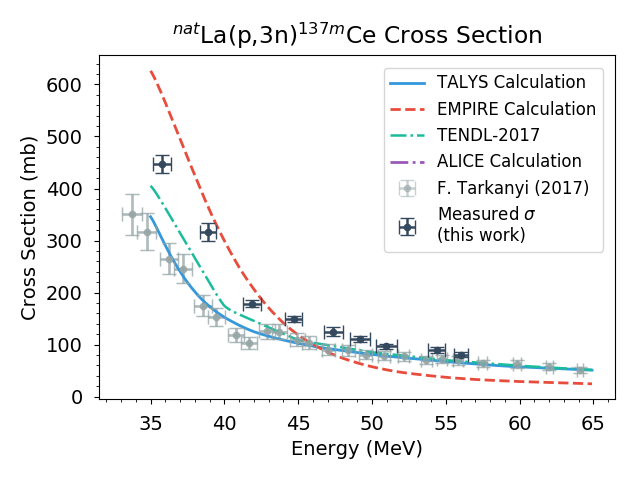
\includegraphics[width=0.32\linewidth]{cross_sections/137CEm.png}\\
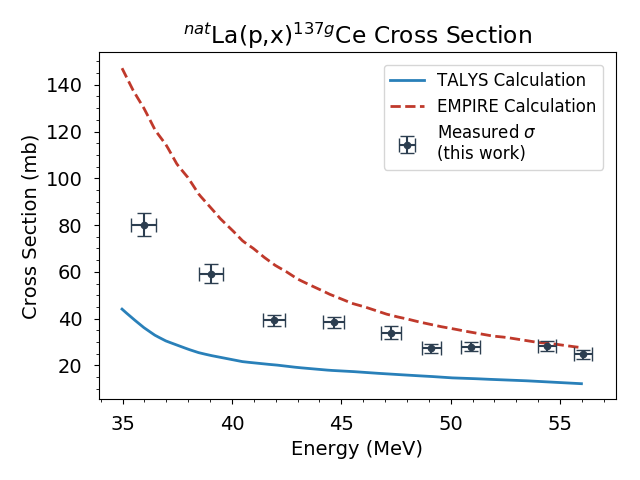
\includegraphics[width=0.32\linewidth]{cross_sections/137CEg.png}
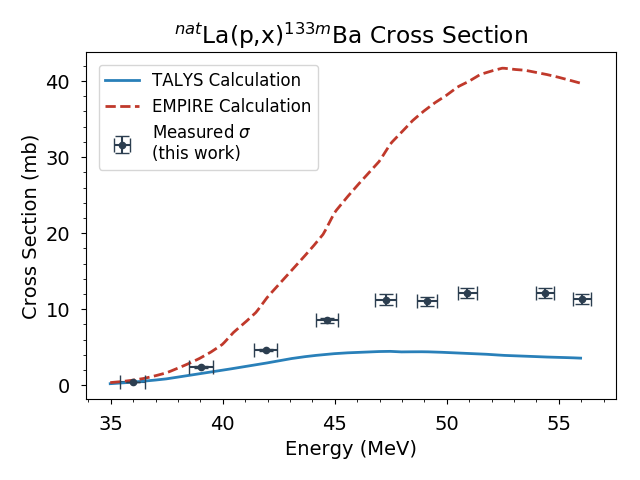
\includegraphics[width=0.32\linewidth]{cross_sections/133BAm.png}
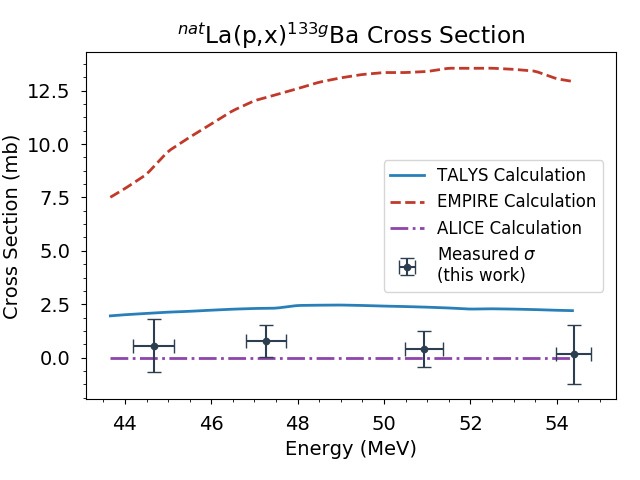
\includegraphics[width=0.32\linewidth]{cross_sections/133BAg.png}\\
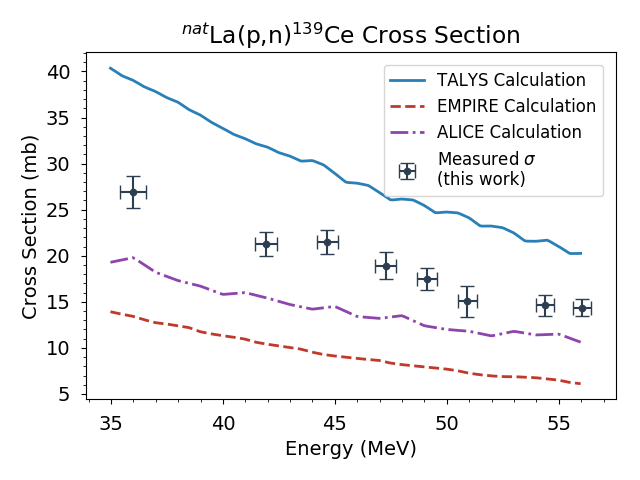
\includegraphics[width=0.32\linewidth]{cross_sections/139CE.png}
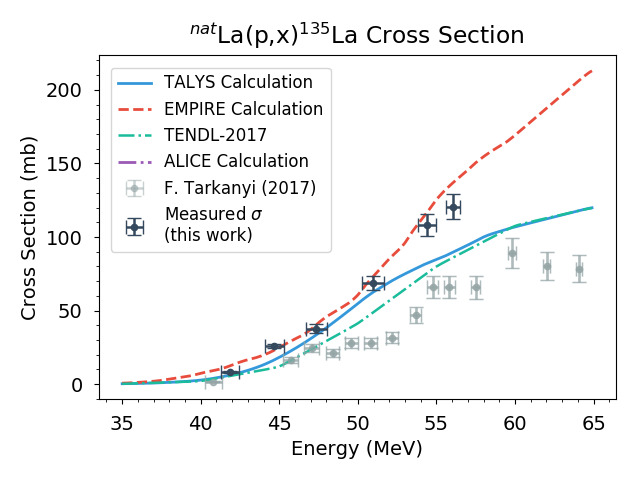
\includegraphics[width=0.32\linewidth]{cross_sections/135LA.png}
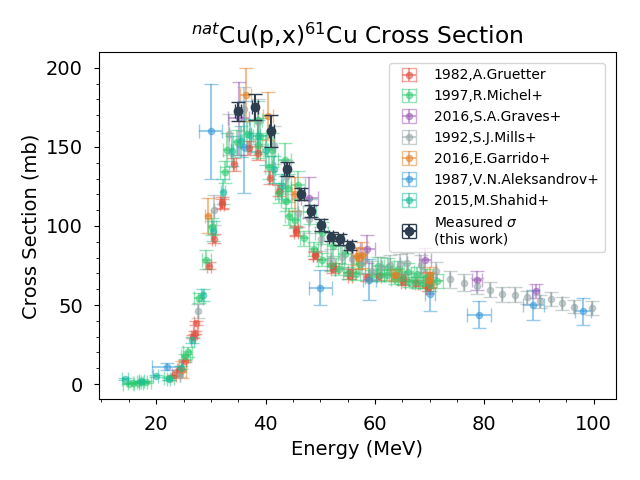
\includegraphics[width=0.32\linewidth]{cross_sections/61CU.png}
\caption{\hspace*{15pt}Measured excitation functions in $^{nat}$La and $^{nat}$Cu (lower right).  TALYS, EMPIRE and ALICE default calculations are shown in solid blue, dashed red, and dashed/dotted purple respectively.}
\end{figure}

%----------------------------------------------------------------------------
\begin{columns}[t,totalwidth=\threecolwid] % Split up the two columns wide column again
\begin{column}{\onecolwid} % The first column within column 2 (column 2.1)
%----------------------------------------------------------------------------
%----------------------------------------------------------------------------

\begin{block}

\small{
\hspace*{50pt}The end-of-beam activity is determined by collecting a spectrum of $\gamma$-rays with a HPGe, identifying and fitting characteristic peaks in the spectrum, and calculating $A_0$ according to

\begin{equation}
A_0 = \frac{\lambda N_c}{(1-e^{-\lambda t_m})e^{-\lambda t_d}I_{\gamma}\epsilon}
\label{eq:activity}
\end{equation}

where $N_c$ is the number of counts in a peak, $t_m$ and $t_d$ are the measurement and decay times, $I_{\gamma}$ is the $\gamma$ emission fraction per decay and $\epsilon$ is the detector efficiency at a particular photo-peak energy.

}

\end{block}

\begin{block}{Energy Assignments}

\small{\hspace*{50pt}The energy centroids (and $\sigma_E$) were first estimated using MCNP, however the estimates using the Anderson-Ziegler stopping power tables proved closer to actual measurements.}

\begin{figure}
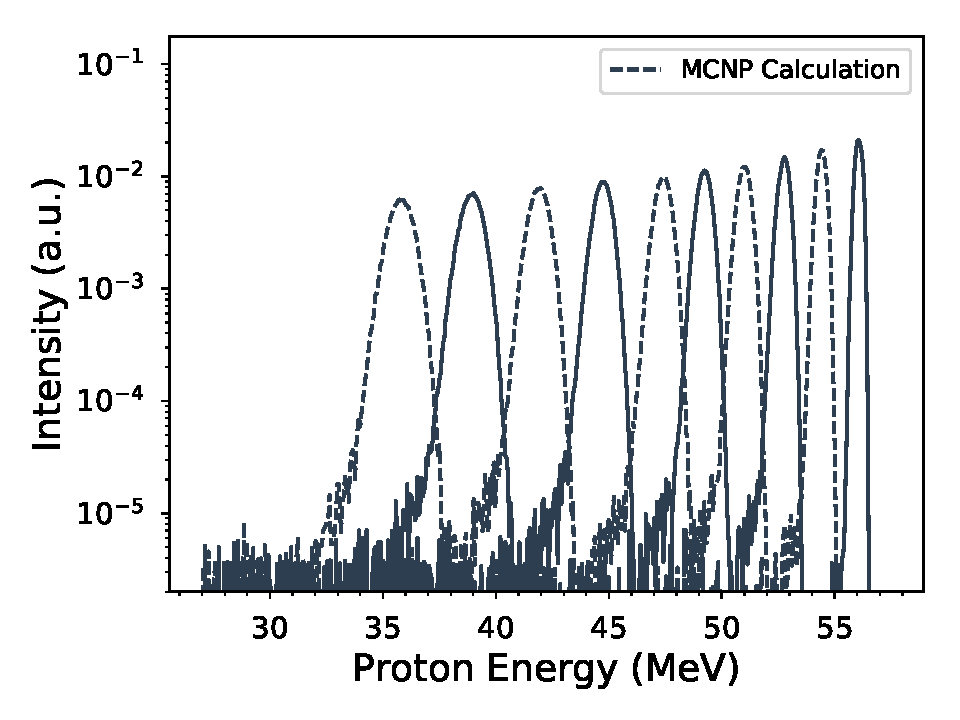
\includegraphics[width=0.8\linewidth]{monitors/La_mcnp_spectrum.pdf}

\caption{\hspace*{15pt}Plot of the proton energy spectra for each lanthanum foil in the target stack.}
\end{figure}

\end{block}

%----------------------------------------------------------------------------
\end{column} % End of column 2.1
\begin{column}{\onecolwid} % The second column within column 2 (column 2.2)
%----------------------------------------------------------------------------
%----------------------------------------------------------------------------

\begin{block}


\small{\hspace*{50pt}The beam current was also calculated using equation 1, but for a known cross-section (instead of known current).  The effective foil density was varied slightly to minimize the variance in beam current measured by the monitor foils.  This procedure simultaneously optimizes the energy assignments and the beam current.}

\begin{figure}
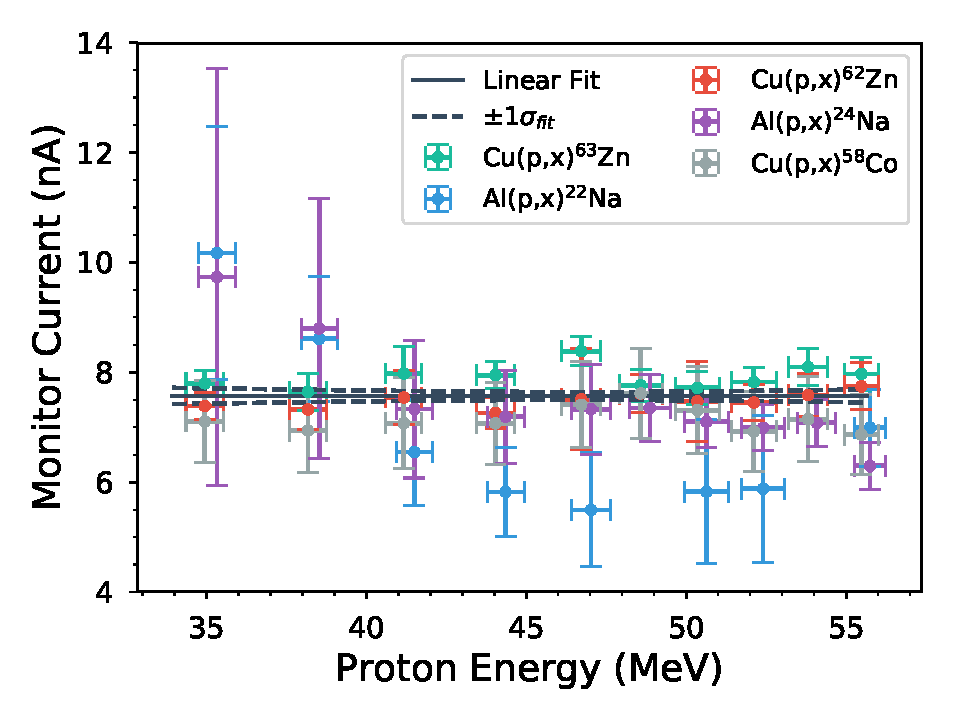
\includegraphics[width=0.8\linewidth]{monitors/current_norm_mcnp.pdf}
\caption{\hspace*{15pt}Plot of the beam current measured by each monitor foil reaction, with a linear fit (and $\pm 1 \sigma$) plotted in black.
}
\end{figure}
\end{block}

\begin{block}{Results}
\small{\hspace*{50pt}The measured cross sections are plotted above, in Figure 3.  The codes TALYS, EMPIRE, and ALICE were ran with default parameters for comparison, although the predictions were quite poor in general.  The $^{nat}$Cu(p,x)$^{61}$Cu cross section was also compared to existing data from the EXFOR database.}
\end{block}

%----------------------------------------------------------------------------
\end{column} % End of column 2.2

\begin{column}{\sepwid}\end{column} % Empty spacer column
\begin{column}{\onecolwid} % The third column

%----------------------------------------------------------------------------
%   RIGHT
%----------------------------------------------------------------------------



%----------------------------------------------------------------------------
%   REFERENCES
%----------------------------------------------------------------------------
\begin{block}{References}
\nocite{*} % Insert publications even if they are not cited in the poster
\small{\bibliographystyle{unsrt}
\footnotesize
\bibliography{LaCe.bib}}
\end{block}
%----------------------------------------------------------------------------
%   ACKNOWLEDGEMENTS
%----------------------------------------------------------------------------
\begin{block}{Acknowledgements}
\small{\rmfamily{\hspace*{50pt}We wish to acknowledge our thanks to the operators of the 88" cyclotron: Brien Ninemire, Nick Brickner, Tom Gimpel and Scott Small for their efforts in setting a new "high-water mark" for the maximum proton energy extracted from the machine.  This work has been performed under the auspices of the U.S. Department of Energy by Lawrence Berkeley National Laboratory under contract No. LAB16-1588 NSD.}} \\
\end{block}
%----------------------------------------------------------------------------
%----------------------------------------------------------------------------

\begin{itemize}
\item Email: \href{mailto:jmorrell@berkeley.edu}{jmorrell@berkeley.edu}
\end{itemize}

%----------------------------------------------------------------------------
\end{column} % End of the third column

\end{columns} % End of the split of column 2
\end{column} % End of the second column

\end{columns} % End of all the columns in the poster
\end{frame} % End of the enclosing frame
\end{document}
              
            